\documentclass[12pt,t]{beamer}
% \documentclass[t]{beamer}

\usepackage{pgfpages}
\usepackage{pgffor}
%\pgfpagesuselayout{4 on 1}[a4paper,landscape]

%\pagestyle{empty} % descomentar para impresión muy blanca

\usepackage[utf8]{inputenc}
\usepackage[spanish]{babel}
\usepackage{verbatim}
\usepackage{hyperref}
\usepackage{amsfonts,amssymb,amsmath,amsthm, wasysym}
\usepackage{listings}
\usepackage[T1]{fontenc}        
\usepackage{pgf}
%\usepackage{epsdice}
\usepackage{pgfpages}
\usepackage{tikz}
%\usetikzlibrary{arrows,shapes,plotmarks,backgrounds,trees,positioning}
%\usetikzlibrary{decorations.pathmorphing,calc,snakes}
%\usepackage{marvosym}
%
\usetheme[hideothersubsections,left]{Marburg}
\usecolortheme{sidebartab}
\useinnertheme[shadow]{rounded}
% \useoutertheme[footline=empty,subsection=true,compress]{infolines}
% \useoutertheme[footline=empty,subsection=true,compress]{miniframes}
% \usefonttheme{serif}

\setbeamertemplate{caption}[numbered]
\setbeamertemplate{navigation symbols}{}


\newcommand{\red}[1]{\textcolor{red}{#1}}
\newcommand{\green}[1]{\textcolor{green}{#1}}
\newcommand{\blue}[1]{\textcolor{blue}{#1}}
\newcommand{\gray}[1]{\textcolor{gray}{#1}}
\renewcommand{\emph}[1]{{\color{red}#1}}

\setbeamertemplate{frametitle}
{\begin{centering}
\medskip
\color{blue}
\textbf{\insertframetitle}
\medskip
\end{centering}
}
\usecolortheme{rose}
\usecolortheme{dolphin}
\mode<presentation>


\newcommand{\CC}{\mathbb{C}}
\newcommand{\RR}{\mathbb{R}}
\newcommand{\ZZ}{\mathbb{Z}}
\newcommand{\NN}{\mathbb{N}}
\newcommand{\KK}{\mathbb{K}}
\newcommand{\MM}{\mathcal{M}}
%\newcommand{\dbinom}{\displaystyle\binom}

\newcommand{\limn}{{\displaystyle \lim_{n\to\infty}}}
\renewcommand{\leq}{\leqslant}
\renewcommand{\geq}{\geqslant}
\def\tendeix{{\displaystyle\mathop{\longrightarrow}_{\scriptscriptstyle
n\to\infty}}}

\newcommand{\matriu}[1]{\left(\begin{matrix} #1 \end{matrix}\right)}

% \newcommand{\qed}{\hbox{}\nobreak\hfill\vrule width 1.4mm height 1.4mm depth 0mm
%     \par \goodbreak \smallskip}
%
% %
\theoremstyle{plain}
\newtheorem{teorema}{Teorema}
\newtheorem{prop}{Proposición}
\newtheorem{cor}{Corolario}
\theoremstyle{definition}
\newtheorem{Ejemplo}{Ejemplo}
\newtheorem{exerc}{Ejercicio}
\newtheorem{defin}{Definición}
\newtheorem{obs}{Observación}

\newcounter{seccions}
\newcommand{\seccio}[1]{\addtocounter{seccions}{1}
\medskip\par\noindent\textbf{\theseccions.
#1}\smallskip\par }

\newcommand{\EM}{\Omega}
\newcommand{\PP}{\mathcal{P}}

\title[\red{Matemáticas III GINF}]{}
\author[]{}
\date{}



\usepackage{Sweave}
\begin{document}
\Sconcordance{concordance:EstimacioPuntual_notas_clase.tex:EstimacioPuntual_notas_clase.Rnw:%
1 421 1 48 0 12 1 28 0 111 1 6 0 518 1 4 0 9 1 7 0 283 1 6 0 32 1}

\beamertemplatedotitem

\lstset{backgroundcolor=\color{green!50}}
\lstset{breaklines=true}
\lstset{basicstyle=\ttfamily}


\section{Estimación puntual}

\begin{frame}
\vfill
\begin{center}
\gray{\LARGE Estimación puntual}
\end{center}
\vfill
\end{frame}






\subsection{Definiciones básicas}


\begin{frame}
\frametitle{Estadística inferencial}

El problema usual de la \emph{estadística inferencial} es:

\begin{itemize}

\item Queremos conocer el valor de una característica en una población
\medskip

\item No podemos medir esta característica en todos los individuos de la población
\medskip

\item Extraemos una muestra  aleatoria de la población,  medimos la característica en los  individuos de esta muestra e  \emph{inferimos} el valor de la característica para la toda la población

\begin{itemize}
\item ¿Cómo lo tenemos que hacer?
\item ¿Cómo tenemos que hacer la muestra?
\item ¿Qué información podemos inferir?
\end{itemize}
\end{itemize}
\end{frame}



\begin{frame}
\frametitle{Ejemplos}

\begin{center}
\hspace*{-0.5cm}

\includegraphics[width=1.1\linewidth]{plagiUIB1.jpg}\bigskip

\hspace*{-0.5cm}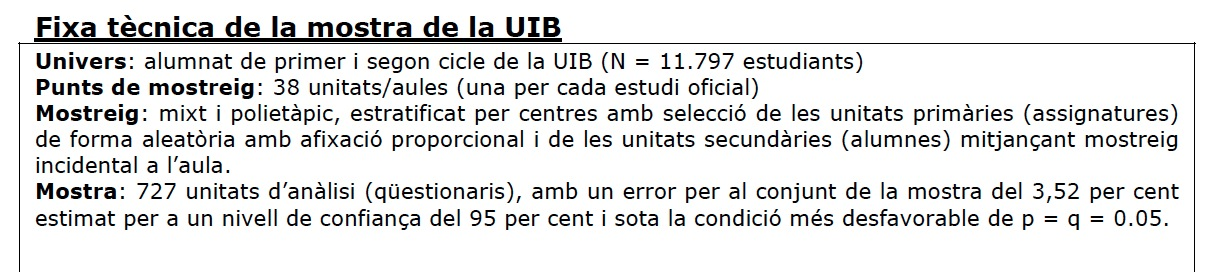
\includegraphics[width=1.1\linewidth]{plagiUIB2.jpg}
\end{center}
\end{frame}


%
%\begin{frame}
%\frametitle{Ejemplos}
%\vspace*{-0.5cm}
%
%\begin{center}
%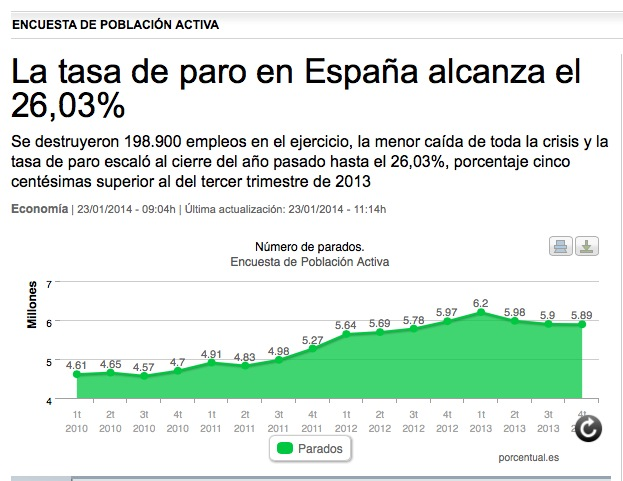
\includegraphics[width=\linewidth]{paro.jpg}
%\end{center}
%\end{frame}

\begin{frame}
\frametitle{Ejemplos}


\begin{center}

\includegraphics[width=\linewidth]{vacuna1.jpg}\medskip

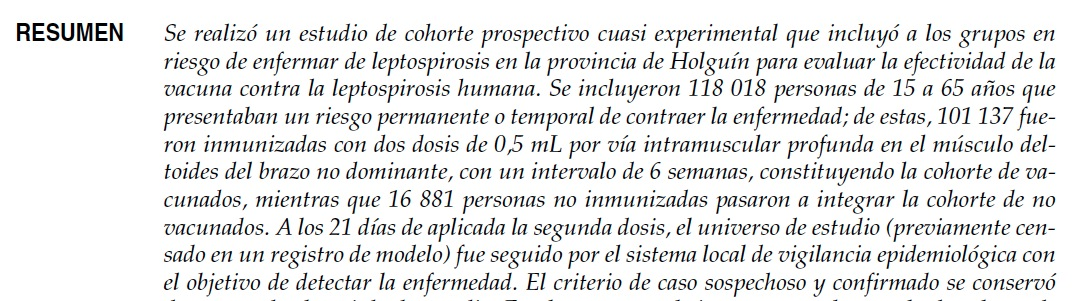
\includegraphics[width=\linewidth]{vacuna2.jpg}
\end{center}


{\footnotesize \url{http://www.scielosp.org/pdf/rpsp/v8n6/3956.pdf}}
\end{frame}

\begin{frame}
\frametitle{Definiciones básicas}

\emph{Muestra aleatoria simple (m.a.s.) de tamaño $n$:} De una población de $N$ individuos, repetimos $n$ veces el proceso   consistente en escoger equiprobablemente un individuo de la población; \textit{los individuos escogidos se pueden repetir}
\bigskip

\blue{Ejemplo:} Escogemos  al azar $n$ estudiantes de la UIB (con reposición) para medirles la estatura
\bigskip

De esta manera, todas las muestras posibles de $n$ individuos (posiblemente repetidos: \emph{multiconjuntos}) tienen la misma probabilidad
\bigskip

%\href{http://www.latex-project.org/}{latex project}
\emph{\bf Leeros la \href{https://aprender-uib.github.io/AprendeR2/chap-muestreo.html}{lección 2 de AprendeR2} sobre muestreo}
\end{frame}


\begin{frame}
\frametitle{Definiciones básicas}

\emph{Estadístico} (\emph{Estimador puntual}): Una función que aplicada a una muestra nos permite \emph{estimar} un valor que queramos conocer sobre  toda la población
\bigskip

\blue{Ejemplo:} La media de les estaturas  de una muestra de estudiantes de la UIB nos permite estimar la media de les alturas de todos los   estudiantes de la UIB
\bigskip

\end{frame}

\begin{frame}
\frametitle{Formalmente}

Una \emph{m.a.s.\ de tamaño $n$} (de una v.a.\ $X$) es
\begin{itemize}
\item  un conjunto de $n$ copias \blue{independientes} de $X$, o

\item un conjunto de $n$ variables aleatorias  \blue{independientes} $X_1,\ldots,X_n$, todas con la distribución de  $X$
\end{itemize}
\medskip


\blue{Ejemplo:} Sea $X$ la v.a.\ ``escogemos un estudiante de la UIB y le medimos la altura''. Una m.a.s.\ de $X$ de tamaño $n$ serán $n$ copias independientes $X_1,\ldots,X_n$ de esta $X$.
\bigskip


Una \emph{realización} de una m.a.s.\ son los $n$ valores $x_1,\ldots,x_n$ que  toman las v.a.\ $X_1,\ldots,X_n$

\end{frame}


\begin{frame}
\frametitle{Formalmente}

Un  \emph{estadístico} $T$ es una función aplicada a la muestra $X_1,\ldots,X_n$:
$$
T=f(X_1,\ldots,X_n)
$$
Este estadístico se aplica a les realizaciones  de la muestra
\medskip

\blue{Ejemplo:} La \emph{media muestral} de una m.a.s.\ $X_1,\ldots,X_n$ de tamaño $n$ es 
$$
\overline{X}:=\frac{X_1+\cdots+X_n}{n}
$$
Estima $E(X)$
\medskip

\blue{Ejemplo:} La media muestral de las alturas de una
realización de una m.a.s.\ de  las alturas  de estudiantes estima  la altura media de un estudiante de la UIB.




\end{frame}


\begin{frame}
\frametitle{Formalmente}

Un  \emph{estadístico} $T$ es una función aplicada a la muestra $X_1,\ldots,X_n$
$$
T=f(X_1,\ldots,X_n)
$$
\medskip

Así pues, un estadístico es una (otra) variable aleatoria, con distribución, esperanza, etc.
\medskip

La \emph{distribución muestral} de $T$ es la distribución de  esta variable aleatoria.
\medskip

Estudiando  esta distribución muestral, podremos estimar propiedades de $X$ a partir del comportamiento de una muestra
\medskip

\emph{Error estándar de $T$}: desviación típica de $T$


\end{frame}



\begin{frame}
\frametitle{Convenio}

\emph{\bf LOS ESTADÍSTICOS, EN MAYÚSCULAS; las realizaciones, en minúsculas}
\medskip

\blue{Ejemplo:} 
\begin{itemize}
\item $X_1,\ldots,X_n$ una m.a.s.\ y 
$$
\overline{X}:=\frac{X_1+\cdots+X_n}{n}
$$
la media muestral\medskip


\item $x_1,\ldots,x_n$ una realización  de esta  m.a.s.\ y 
$$
\overline{x}:=\frac{x_1+\cdots+x_n}{n}
$$
la media (muestral) de esta realización
\end{itemize}

\end{frame}




\begin{frame}
\frametitle{La vida real}

En la vida real, las muestras aleatorias se toman, casi siempre, sin reposición (es decir sin repetición del mismo individuo de la población).

No son muestras aleatorias simples. pero:
\begin{itemize}
\item Si $N$ es mucho más grande que $n$,  los resultados para una   m.a.s.\ son  (aproximadamente) los mismos,  ya que las  repeticiones son improbables y las variables aleatorias que forman la muestra son prácticamente  independientes.
\smallskip

En estos casos cometeremos el abuso de lenguaje  de decir que es una m.a.s.

\medskip

\item Si $n$ es relativamente grande, se suelen dar  versiones corregidas de los estadísticos
\end{itemize}

\end{frame}


\begin{frame}
\frametitle{La vida real}

\blue{Ejemplo:} La UIB tiene unos 15000 estudiantes


% <<estudiantes_rep,size="tiny",fig.height=4,eval=FALSE>>=
% estudiantes = function(n) {choose(15000,n)/(15000)^n}
% %añsjfañjsdfñlkájsdlkaj
% plot(0:80,estudiantes(0:80), xlim = c(0, 80), 
%      xlab = "n",ylab = "probabilidad",
%      main = "Probabilidad de que si elegimos\n n estudiantes de la UIB sean \n todos distintos",
%      type = "l"


% )
% @

\begin{center}
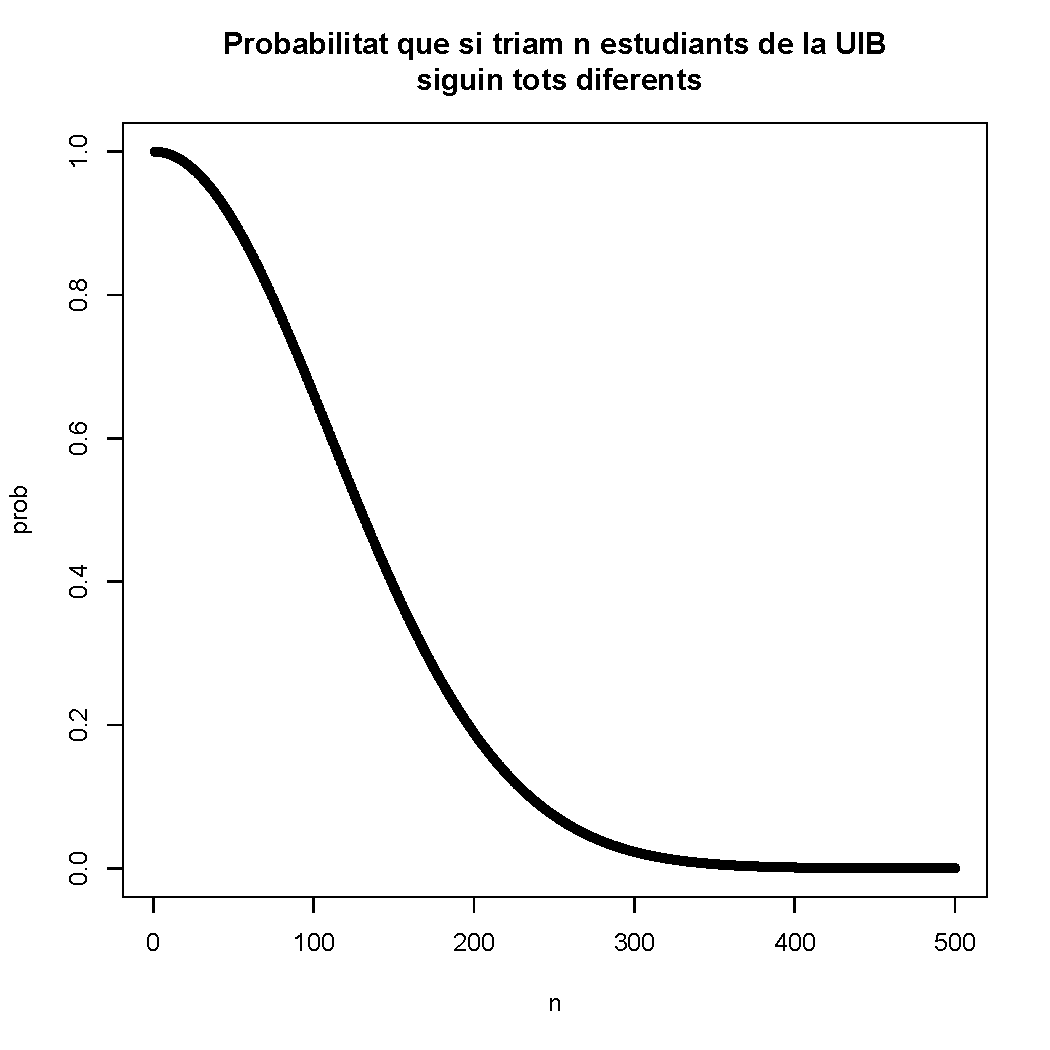
\includegraphics[width=0.8\linewidth]{UIB.pdf}
\end{center}

\end{frame}


%%Concurs1
%La UIB té uns 16000 estudiants. 
%
%a) Quina es la probabilitat que si en triam n a l'atzar, un rere l'altre y con reposició, sean tots diferents?
%b) Definiu una funció de R que, aplicada a n, doni aquesta probabilitat
%c) Calculau la llista $(f(n))_{n=2,150}$ (per aplicar una funció a una llista, si directament no funciona, podeu emprar sapply(llista, funció)). Quin es el nombre màxim d'estudiants que podem triar de manera que la probabilitat que sean tots diferents sea com a mínim del 95\%?
%d) La funció $f$, es aproximadamentelineal, polinòmica o exponencial (o cap de les tres coses) en $n$? En cas afirmatiu, trobau la funció que l'aproxima, y confirmau con un gràfic aquesta aproximació.



\subsection{media muestral}
\begin{frame}
\frametitle{media muestral}

Sea $X_1,\ldots, X_n$ una m.a.s.\ de tamaño $n$ de una v.a.\ $X$ de esperanza $\mu_X$ y desviación típica $\sigma_X$
\medskip

La \emph{media muestral} es
$$
\overline{X}=\frac{X_1+\cdots+X_n}{n}
$$

\begin{teorema}
En estas condiciones
$$
E(\overline{X})=\mu_X,\quad \sigma_{\overline{X}}=\frac{\sigma_X}{\sqrt{n}}
$$
\end{teorema}

 $\sigma_{\overline{X}}$ es el \emph{error estándar} de $\overline{X}$



\end{frame}

\begin{frame}
\frametitle{Media muestral}

$$
\overline{X}=\frac{X_1+\cdots+X_n}{n}
$$
\begin{itemize}
\item es un estimador puntual de $\mu_X$
\medskip

\item \emph{$E(\overline{X})=\mu_X$}
\begin{itemize}
\item El valor esperado de $\overline{X}$ es $\mu_X$
\medskip

\item Si tomamos muchas veces una m.a.s.\ y calculamos la media muestral, el valor medio  de estas medias tiende con mucha probabilidad a ser $\mu_X$
\end{itemize}
\bigskip

\item \emph{$\sigma_{\overline{X}}= \sigma_X/\sqrt{n}$}: la variabilidad de los resultados de $\overline{X}$ tiende a 0  a medida que tomamos muestras más grandes 
\end{itemize}

\end{frame}

\begin{frame}[fragile]
\frametitle{Media muestral}
\vspace*{-2ex}


\begin{Schunk}
\begin{Sinput}
> # tests.txt=notas de un examen  sobre estadística descriptiva 
> notas=read.table("http://bioinfo.uib.es/~recerca/matIII_GIN/notas.txt", header=TRUE)
> str(notas)
\end{Sinput}
\begin{Soutput}
'data.frame':	185 obs. of  1 variable:
 $ x: num  54.5 60.1 53 57.3 54.4 ...
\end{Soutput}
\begin{Sinput}
> mean(notas$x)
\end{Sinput}
\begin{Soutput}
[1] 55.32254
\end{Soutput}
\begin{Sinput}
> set.seed(100)
> medias=replicate(10^4,mean(sample(notas$x,40,rep=TRUE)))
> head(medias)
\end{Sinput}
\begin{Soutput}
[1] 54.72700 55.14975 54.79800 56.43350 54.36725 54.97000
\end{Soutput}
\begin{Sinput}
> mean(medias)
\end{Sinput}
\begin{Soutput}
[1] 55.3281
\end{Soutput}
\begin{Sinput}
> #sd, por ir  deprisa
> c(sd(notas$x)/sqrt(40),sd(medias))
\end{Sinput}
\begin{Soutput}
[1] 0.5209303 0.5252889
\end{Soutput}
\end{Schunk}


\end{frame}

\begin{frame}
\frametitle{Ejemplo}
Se toma  una m.a.s.\ de 10 estudiantes de los estudios del grado de informática (GIN), y se miden sus estaturas. Se obtuvieron estos resultados:

$$
1.62,1.75,1.64,1.69,1.83,1.85,1.72,1.61,1.93, 1.62
$$
Podemos  estimar la estatura media de los estudiantes del GIN:

$$
\overline{x}=\frac{1.62+1.75+1.64+\cdots+1.62}{10}=1.726
$$
¿Cuál es la precisión de esta estimación? 
\break 

``\emph{.....The solution is comming!!!!}" ¡No os perdáis las próximas lecciones!

\end{frame}


\begin{frame}
\frametitle{La combinación lineal de normales es normal}
\begin{teorema}
Si $Y_1,\ldots,Y_n$ son v.a.\ normales independientes, cada $Y_i\sim N(\mu_i,\sigma_i)$, y $a_1,\ldots,a_n,b\in \RR$ entonces
$$
Y=a_1Y_1+\cdots+a_nY_n+b
$$
es una v.a.\ $N(\mu,\sigma)$ con $\mu$ y $\sigma$ las que correspondan:
\begin{itemize}
\item $E(Y)=a_1\cdot\mu_1+\cdots+a_n\cdot\mu_n+b$
\medskip

\item $\sigma(Y)^2=a_1^2\cdot\sigma_1^2+\cdots+a_n^2\cdot\sigma_n^2$
\end{itemize}
\end{teorema}
\end{frame}




\begin{frame}
\frametitle{Caso  en el que $X$  tiene distribución normal}
\begin{teorema}
Sea $X_1,\ldots, X_n$ una m.a.s.\ de una v.a.\ $X$ de esperanza $\mu_X$ y desviación típica $\sigma_X$.
Si $X$ es $N(\mu_X,\sigma_X)$, entonces
$$
\overline{X}\mbox{ es }N\Big(\mu_X,\frac{\sigma_X}{\sqrt{n}}\Big)
$$
y por lo tanto
$$
Z=\frac{\overline{X}-\mu_X}{\frac{\sigma_X}{\sqrt{n}}}\mbox{ es }N(0,1)
$$
\end{teorema}

$Z$ es la \emph{expresión tipificada} de la media muestral

\end{frame}




\begin{frame}
\frametitle{Teorema Central del Límite}
\begin{teorema}
Sea $X_1,\ldots, X_n$ una m.a.s.\ de una v.a.\ $X$ \emph{cualquier} de esperanza $\mu_X$ y desviación típica $\sigma_X$. Cuando $n\to \infty$, 
$$
\overline{X}\to N\Big(\mu_X,\frac{\sigma_X}{\sqrt{n}}\Big)
$$
y por lo tanto
$$
Z=\frac{\overline{X}-\mu_X}{\frac{\sigma_X}{\sqrt{n}}}\to N(0,1)
$$
(estas convergencias se refieren a las distribuciones.)
\end{teorema}
\end{frame}



\begin{frame}
\frametitle{Teorema Central del Límite}

\begin{block}{``Teorema''}
Si $n$ es grande (\emph{$n\geq 30$ o \underline{\textbf{40}}}), 
$\overline{X}$ es aproximadamente normal, con esperanza  $\mu_X$ y desviación típica  $\dfrac{\sigma_X}{\sqrt{n}}$
\end{block}
\bigskip

\blue{Ejemplo:} Tenemos una v.a.\ $X$ de media $\mu_X=3$ y desv. típ. 
$\sigma_X=0.2$. Tomamos  muestras aleatorias  simples de tamaño 50. La distribución de la media muestral $\overline{X}$ es aproximadamente
$$
N\left(3,\frac{0.2}{\sqrt{50}}\right)=N(3,0.0283)
$$
\end{frame}

\begin{frame}[fragile]
\frametitle{Teorema Central del Límite}
\begin{Schunk}
\begin{Sinput}
> # con los datos de las  10000 medias de muestras
> #de tamaño 40  las notas anteriores
> hist(medias,freq=FALSE, main="Histograma 
+  de les medias de 10000 muestras de 40 notas",ylab="Densidad",ylim=c(0,0.8))
> lines(density(medias),lty=2,lwd=2,col="red")
> curve(dnorm(x,mean(notas$x),sd(notas$x)/sqrt(40)),
+  lty=3,lwd=2,col="blue",add=TRUE)
> legend("topright",legend=c("densidad","normal"),
+  lwd=c(2,2),lty=c(2,3),col=c("red","blue"))
\end{Sinput}
\end{Schunk}

\end{frame}


% 
% \begin{frame}
% \frametitle{Teorema Central del Límite}
% \vspace*{-4ex}
% 
% \begin{center}
% 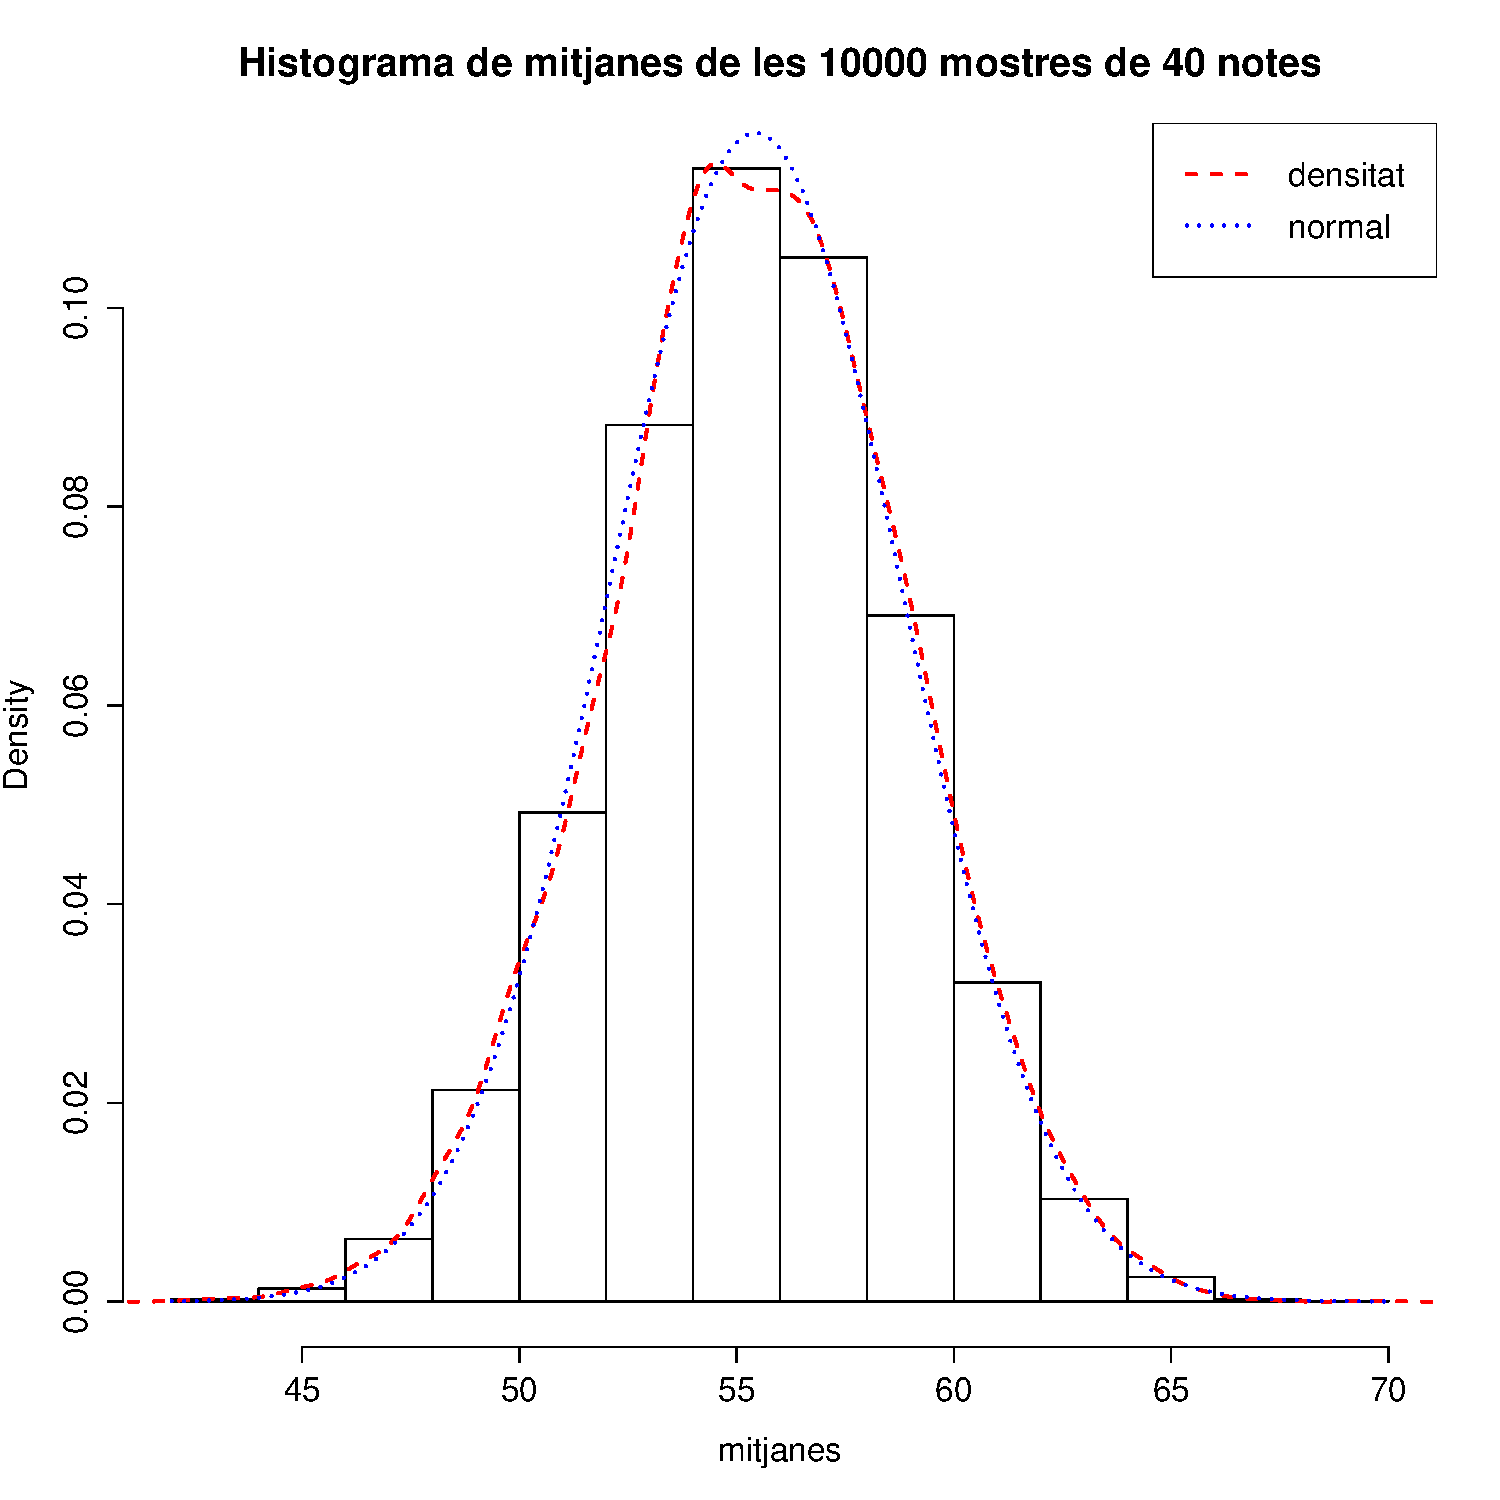
\includegraphics[width=0.8\linewidth]{hist-test}
% \end{center}
% 
% 
% 
% \end{frame}




\begin{frame}
\frametitle{Ejemplo}
\vspace*{-2ex}

El tamaño en megabyte (MB)  de un  tipo de imágenes comprimidas tiene  un  valor medio de   $115$ MB, con una desviación típica de $25$. Tomamos  una m.a.s.\ de $100$ imágenes de este tipo.
\medskip

\blue{¿Cuál es la probabilidad de que la media muestral del tamaño de los ficheros  sea $\leq 110$ MB?}
\medskip

$\displaystyle Z=\frac{\overline{X}-\mu_{X}}{\frac{\sigma_{X}}{\sqrt{n}}}=
\frac{\overline{X}-115}{2.5}$ es (\red{aproximadamente}) $N(0,1)$
\medskip

$\begin{array}{rl}
P(\overline{X}\leq 110)  &\displaystyle= P\Big(Z\leq \frac{110-115}{2.5}\Big)= P(Z\leq -2)\\[2ex]
& \displaystyle=0.0228
\end{array}$


\end{frame}



\begin{frame}
\vspace*{-2ex}

\frametitle{Ejemplo}

El tamaño en megabyte (MB)  de un  tipo de imágenes comprimidas tiene  un  valor medio de   $115$ MB, con una desviación típica de $25$. Tomamos  una m.a.s.\ de $100$ imágenes de este tipo.
\medskip

\blue{¿Cuál es la probabilidad de que la media muestral del tamaño de las imágenes esté entre $113$ MB y $117$ MB?}
\medskip


\end{frame}








\begin{frame}
\frametitle{Media muestral en muestras sin reposición}

Sea $X_1,\ldots, X_n$ una m.a.\ \emph{sin  reposición} de tamaño $n$ de una v.a.\ $X$ de esperanza $\mu_X$ y desviación típica $\sigma_X$. 
\medskip

Si $n$ es  pequeño en relación al tamaño $N$ de la población, todo lo que hemos contado funciona (aproximadamente)
\medskip

Si $n$ es grande en relación a $N$, entonces
$$
E(\overline{X})=\mu_X,\quad \sigma_{\overline{X}}=\frac{\sigma_X}{\sqrt{n}}\cdot\red{\sqrt{\frac{N-n}{N-1}}}
$$
(\emph{factor de población finita})
\medskip

El T.C.L. ya no funciona exactamente en este último caso
\end{frame}

\subsection{Proporción  muestral}
\begin{frame}
\frametitle{Proporción  muestral}

Sea $X$ una v.a.\ Bernoulli de parámetro  $p_X$ (1 éxito, 0 fracaso). Sea $X_1,\ldots,X_n$ una m.a.s.\ de tamaño $n$ de $X$. 
\medskip

$S=\sum_{i=1}^n X_i$ es el nombre de éxitos observados
es $B(n,p)$.
\medskip

La \emph{proporción muestral} es 
$$
\widehat{p}_X=\frac{S}{n}
$$
y es un estimador de $p_X$
\medskip

Notemos que $\widehat{p}_X$ es un caso particular de $\overline{X}$, por lo que todo lo que hemos dicho para medias muestrales es cierto para proporciones muestrales.

\end{frame}


\begin{frame}
\frametitle{Proporción  muestral}
$\widehat{p}_X=\dfrac{S}{n}$
\medskip

\begin{itemize}
\item $E(\widehat{p}_X)=p_X$
\medskip


\item $\displaystyle \sigma_{\widehat{p}_X}=\sqrt{\frac{p_X(1-p_X)}{n}}$, l'\emph{error estándar} de la proporción muestral
\medskip

\item Si la muestra es sin reposición y $n$ es relativamente grande,
$\displaystyle\sigma_{\widehat{p}_X}=\sqrt{\frac{p_X(1-p_X)}{n}}\cdot\red{\sqrt{\frac{N-n}{N-1}}}$
\end{itemize}

\end{frame}


\begin{frame}
\frametitle{Proporción  muestral}
\vspace*{-2ex}

Por el  T.C.L.:

\begin{block}{``Teorema''}
Si $n$ es grande (\emph{$n\geq 30$ o \underline{\textbf{40}}}) y la muestra es aleatoria simple, 
$$
\frac{\widehat{p}_X-p_X}{\sqrt{\frac{{p}_X(1-{p}_X)}{n}}}\approx N(0,1)
$$
\end{block}

\end{frame}


\begin{frame}
\frametitle{Ejemplo}
\vspace*{-2ex}

En una muestra aleatoria de 60 estudiantes de la UIB del curso 2013-14, 37 son mujeres. Estimar la fracción de mujeres entre los estudiantes de la UIB
\medskip

$$
\frac{37}{60}=0.6167
$$
\vspace*{-2ex}

\begin{center}
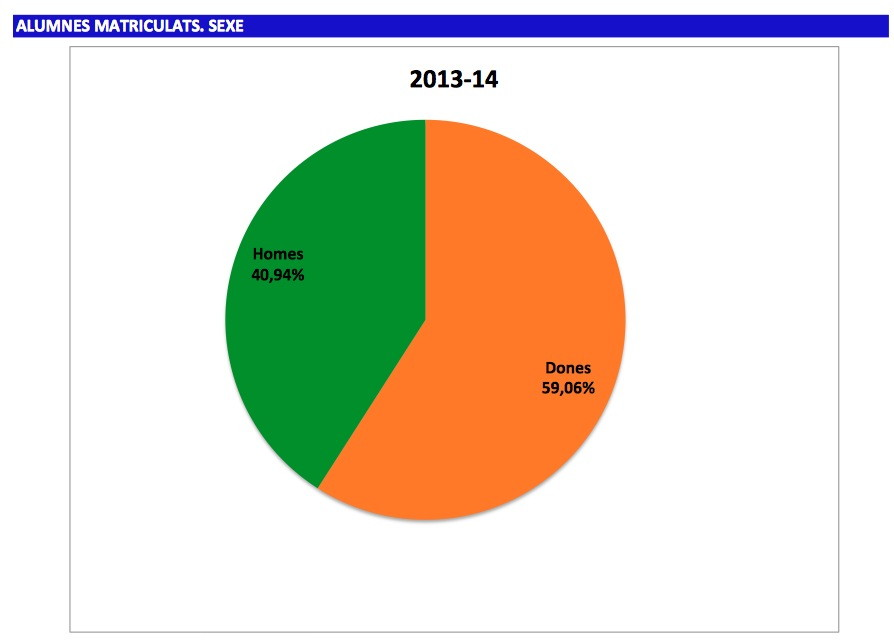
\includegraphics[width=0.7\linewidth]{sexeUIB}
\end{center}


\end{frame}


\begin{frame}
\frametitle{Ejemplo}
\vspace*{-2ex}

\blue{Un  59\% de los estudiantes de la UIB son  mujeres. Si tomamos una m.a.s.\ de 60 estudiantes, ¿cuál es la probabilidad que la proporción muestral de mujeres sea superior al 61\%?}
\medskip 


   
\end{frame}


\subsection{Varianza muestral}

\begin{frame}
\frametitle{Varianza muestral}

Sea $X_1,\ldots, X_n$ una m.a.s.\ de tamaño $n$ de una v.a.\ $X$ de esperanza $\mu_X$ y desviación típica $\sigma_X$
\medskip

La \emph{varianza muestral} es
$$
\widetilde{S}_{X}^2=\frac{\sum_{i=1}^n (X_{i}-\overline{X})^2}{n-1}
$$
La \emph{desviación típica muestral} es 
$$
\widetilde{S}_{X}=+\sqrt{\widetilde{S}_{X}^2}
$$
A mes, escriurem
$$
S^2_{X}=\frac{\sum_{i=1}^n (X_{i}-\overline{X})^2}{n}=\frac{(n-1)}{n}\widetilde{S}^2_{X}\quad\mbox{ y }\quad S_X=+\sqrt{S_X^2}
$$
\end{frame}


\begin{frame}
\frametitle{Varianza muestral: Propiedades}
\begin{itemize}
\item $\displaystyle S^2_X=\frac{\sum_{i=1}^n (X_{i}-\overline{X})^2}{n}=\left(\frac{\sum_{i=1}^n
X_{i}^2}{n}-\overline{X}^2\right)$\medskip

\item $\displaystyle \widetilde{S}_{X}^2=\frac{n}{n-1}\left(\frac{\sum_{i=1}^n
X_{i}^2}{n}-\overline{X}^2\right)$\medskip

\end{itemize}


\begin{teorema}
Si la v.a.\ $X$ es normal, entonces $E(\widetilde{S}_{X}^2)=\sigma_{X}^2$ y 
la v.a.
$$
\frac{(n-1)\widetilde{S}_{X}^2}{\sigma_{X}^2}
$$
té distribución $\chi_{n-1}^2$
\end{teorema}
\end{frame}


\begin{frame}
\frametitle{La distribución $\chi_n^2$}

La distribución $\chi_n^2$ ($\chi$: en catalán, \emph{khi}; en castellano, \emph{ji}; en inglés, \emph{chi}), on $n$  es un parámetro llamado  \emph{grados de libertad}:
\begin{itemize}
\item es la de 
$$
X=Z_{1}^{2}+Z_{2}^{2}+\cdots +Z_{n}^{2}
$$ 
on  $Z_{1},Z_{2},\ldots, Z_{n}$ son v.a.\  independientes  $N(0,1)$
\medskip

\item Su función de densidad es:
$$
f_{\chi_n^2}(x)={\frac{1}{2^{n/2} \Gamma (n/2)}} x^{(n/2)-1} e^{-x/2}\quad\mbox{ si $x\geq 0$}
$$
on $\Gamma(x)=\int_{0}^{\infty} t^{x-1}e^{-t}\, dt$ si $x> 0$

\end{itemize}
\end{frame}


\begin{frame}
\frametitle{La distribución $\chi_n^2$}

\begin{itemize}
\item La distribución está tabulada (\emph{Tenéis unas tablas en Aula Digital}), y con R es \texttt{chisq}
\bigskip

\item Si $X_{\chi_n^2}$ es una v.a.\ con distribución  $\chi_n^2$,
$$E(X_{\chi_n^2})=n,\quad Var(X_{\chi_n^2})=2 n$$
\medskip

\item ${\chi_n^2}$ se aproxima a una distribución normal $N(n,\sqrt{2n})$ para  $n$ grande
($n>40$ o $50$) 
\end{itemize}

\end{frame}

\begin{frame}
\frametitle{La distribución $\chi_n^2$}
\vspace*{-1cm}

\begin{center}
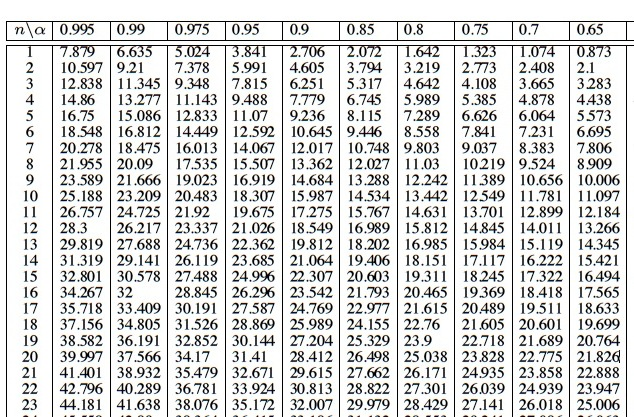
\includegraphics[width=\linewidth]{taulachi.jpg}
\end{center}

$F_{\chi_{10}^2}(25.188)=0.995$,\  $F_{\chi_{20}^2}(26.5)\approx 0.85$
%\quad  \blue{¡haced el test!}

\end{frame}


\begin{frame}
\frametitle{La distribución $\chi_n^2$}
\vspace*{-1cm}

\begin{center}
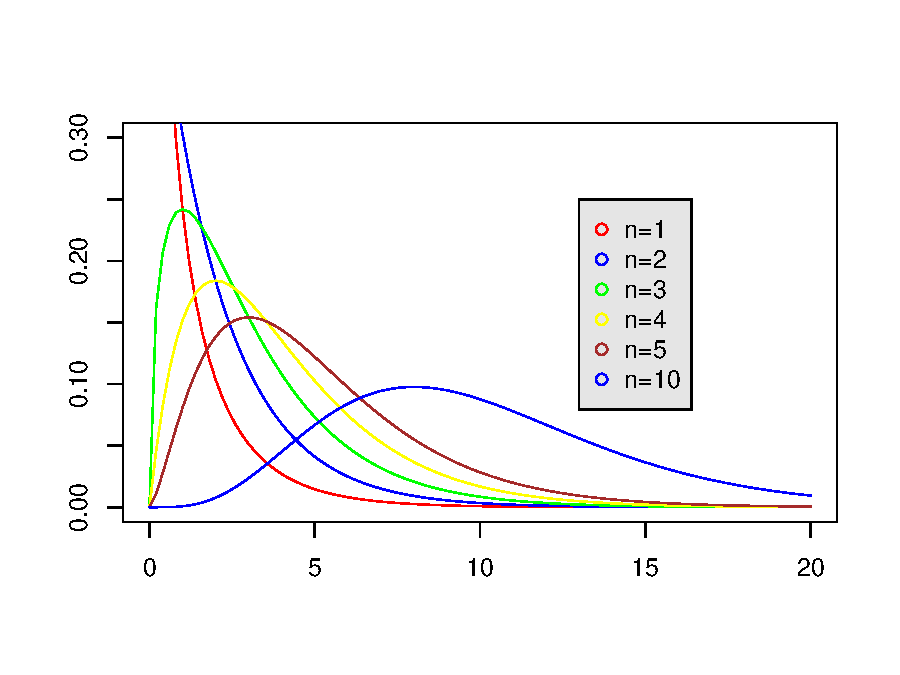
\includegraphics[width=\linewidth]{./dibujos-001}

Función  de densidad de $\chi^2_n$ para  algún  $n$
\end{center}
\end{frame}

\begin{frame}
\frametitle{Ejemplo}
\vspace*{-2ex}

Supongamos que  el  aumento  diario del la ocupación de una granja de  discos duros medido  en Gigas sigue distribución normal con desviación típica $1.7$. Se toma una muestras de 12 discos. Supongamos que esta  muestra es pequeña respecto del total de la población de la granja de discos.
\medskip

\blue{¿Cual es  la probabilidad de que la desviación típica muestral
sea $\leq 2.5$?}
\medskip

Sea $X$= aumento diario en Gigas de un disco duro elegido al azar. 
Sabemos que $\sigma_{X}^2=(1.7)^2=2.89$. Como que $X$ es normal
 y $n=12$, tenemos que
 
$$
\frac{11\cdot \widetilde{S}_{X}^2}{2.89}=\frac{(n-1)\widetilde{S}_{X}^2}{\sigma_{X}^2}\sim \chi^2_{11}
$$

        
\end{frame}


\begin{frame}
\frametitle{Ejemplo}
\vspace*{-2ex}

Supongamos que  el  aumento  diario del la ocupación de una granja de  discos duros medido  en Gigas sigue distribución normal con desviación típica $1.7$. Se toma una muestras de 12 discos. Supongamos que esta  muestra es pequeña respecto del total de la población de la granja de discos.
\medskip

\blue{¿Probabilidad de que la desviación típica muestral
sea $\leq 2.5$?}
\medskip

$\dfrac{11\widetilde{S}_{X}^2}{2.89}\sim \chi^2_{11}$
\medskip

$\begin{array}{l}
\displaystyle P(\widetilde{S}_{X}<2.5)= P\left(\widetilde{S}_{X}^2<2.5^2\right)\\
\quad \displaystyle =P\left(\frac{11\cdot \widetilde{S}_{X}^2}{2.89}<\frac{11
\cdot 2.5^2}{2.89}\right)= P(\chi_{11}^2<23.79)\\
\only<2>{\quad\displaystyle=\mbox{\texttt{pchisq(23.7889,11)}}=0.986}
\only<3>{\quad \displaystyle \approx P(\chi_{11}^2<24.725)=0.99}
\end{array}$
        
\end{frame}


\subsection{Propiedades de los estimadores}


\begin{frame}
\frametitle{Estimadores insesgado}

¿Cuándo un estimador es bueno?
\medskip

Un estimador puntual $\widehat{\theta}$ de un parámetro  poblacional
$\theta$ es  \emph{insesgado, no sesgado o sin sesgo} cuando su valor esperado es precisamente el valor del parámetro:
$$
E(\widehat{\theta})=\theta
$$ 
Entonces se dice que el estimador puntual es \emph{no sesgado}.
\medskip

El  \emph{sesgo} de $\widehat{\theta}$ es $E(\widehat{\theta})-\theta$

\end{frame}


\begin{frame}
\frametitle{Estimadores no segados}


\blue{Ejemplos}

\begin{itemize}
\item $E(\overline{X})=\mu_X$: $\overline{X}$ es estimador no sesgado de $\mu_X$
\medskip

\item $E(\widehat{p}_X)=p_X$: $\widehat{p}_X$ es estimador no sesgado de $p_X$
\medskip

\item $E(\widetilde{S}_{X}^2)=\sigma_X^2$ si $X$ es normal: $\widetilde{S}_{X}^2$ es estimador no sesgado de $\sigma_X^2$ si  $X$ es normal
\medskip

\item $E({S}_{X}^2)=\dfrac{n-1}{n}\sigma_X^2$ si $X$ es normal; por lo tanto 
\emph{${S}_{X}^2$ es sesgado}, con sesgo
$$
E({S}_{X}^2)-\sigma_X^2=\dfrac{n-1}{n}\sigma_X^2-\sigma_X^2=-\dfrac{\sigma_X^2}{n}\ \tendeix\ 0
$$

\end{itemize}

\end{frame}


\begin{frame}
\frametitle{Estimadores eficientes}

¿Cuando un estimador  un estimador es \emph{bueno}?
\medskip

Cuando es no segado y tiene poca variabilidad  (así es más probable que aplicado a una m.a.s.\ de un valor más cercano al valor esperado)
\medskip

\emph{Error estándar de un estimador $\widehat{\theta}$}:  es su desviación típica
$$\sigma_{\widehat{\theta}}=\sqrt{Var(\widehat{\theta})}$$
\medskip

\end{frame}


\begin{frame}
\frametitle{Estimadores eficientes}

Dados dos estimadores $\widehat{\theta}_1$, $\widehat{\theta}_2$ no sesgados (o con sesgo  que $\tendeix 0$) del mismo parámetro  $\theta$, diremos que 
\begin{center}
$\widehat{\theta}_1$ es \emph{más eficiente} que $\widehat{\theta}_2$
\end{center}
 cuando $$\sigma_{\widehat{\theta}_1}< \sigma_{\widehat{\theta}_2},$$  es decir, cuando $$Var(\widehat{\theta}_1)< Var(\widehat{\theta}_2)$$


\end{frame}


\begin{frame}
\frametitle{Estimadores eficientes}

\blue{Ejemplo}: Sea $X$ una v.a.\ con media $\mu_X$ y desviación típica $\sigma_X$
\medskip

Consideremos la mediana $Me=Q_{0.5}$ de la realización de una m.a.s.\ de $X$ como estimador puntual de $\mu_X$
\medskip

Si $X$ es normal, 
$$
\begin{array}{l}
E(Me)=\mu_X,\\
\displaystyle  Var(Me)\approx \frac{\pi}{2}
     \frac{\sigma_{X}^2}{n}\approx \frac{1.57 \sigma_{X}^2}{n}=1.57\cdot Var(\overline{X})
\end{array}
$$
Por  lo tanto, $Me$ es un estimador no sesgado de   $\mu_X$, pero menos eficiente que $\overline{X}$



\end{frame}


\begin{frame}
\frametitle{Estimadores  eficientes}

\begin{itemize}
\item Si la población es normal, la media muestral es el estimador
no sesgado más eficiente de la media poblacional
\medskip

\item Si la población es Bernoulli, la proporción muestral es el estimador
no sesgado más eficiente de la proporción poblacional
\medskip

\item Si la población es normal, la varianza muestral es el estimador
no sesgado  más eficiente de la varianza poblacional
 \end{itemize}




\end{frame}


\begin{frame}
\frametitle{Estimadores  eficientes}

Como hemos visto  si la población es normal, la varianza muestral es el estimador
no sesgado  más eficiente de la varianza poblacional
\medskip

El estimador ``varianza''
$$
S_X^2=\frac{(n-1)}{n} \widetilde{S}_X^2
$$   
aunque sea   más eficiente, tiene sesgo $\tendeix 0$
\medskip

Si $n$ es pequeño ($\leq 30$ o 40), es mejor utilizar  la varianza muestral $\widetilde{S}_X^2$ para estimar la varianza, ya que el sesgo influye, pero si $n$ es grande, el sesgo ya no es tan importante y se puede utilizar $S_X^2$


\end{frame}



\begin{frame}
\frametitle{Ejemplo: Estimación de poblaciones }

Tenemos una población numerada $1,2,\ldots,N$\medskip

Tomamos  una m.a.s. $x_1,\ldots,x_n$; sea
$m=\max(x_1,\ldots,x_n)$
\medskip

\begin{block}{Teorema}
El estimador no segado más eficiente de $N$ es
$$
\widehat{N}=m+\frac{m-n}{n}
$$
\end{block}
\bigskip


Un problema de relevancia histórica:

{\scriptsize \url{http://en.wikipedia.org/wiki/German_tank_problem}}

\end{frame}



\begin{frame}[fragile]
\frametitle{Ejemplo: Estimación de poblaciones }
\vspace*{-2ex}

\blue{Ejemplo:}
Sentados en una terraza de un bar del Paseo Marítimo de Palma hemos anotado el número de licencia de los 40 primeros taxis que hemos visto pasar:
\vspace*{-1ex}


\begin{Schunk}
\begin{Sinput}
> taxis=c(1217,600,883,1026,150,715,297,137,508,134,38,961,538,1154,
+         314,1121,823,158,940,99,977,286,1006,1207,264,1183,1120,
+         498,606,566,1239,860,114,701,381,836,561,494,858,187)
\end{Sinput}
\end{Schunk}

\vspace*{-1ex}

Supondremos que estas observaciones son  una m.a.s. de los taxis de Palma. Entonces, estimamos  que el número de taxis de Palma es
\vspace*{-1ex}
\begin{Schunk}
\begin{Sinput}
> N=max(taxis)+(max(taxis)-length(taxis))/length(taxis)
> N
\end{Sinput}
\begin{Soutput}
[1] 1268.975
\end{Soutput}
\end{Schunk}
\vspace*{-1ex}
En realidad, hay  1246 
\medskip
{\tiny \url{http://www.caib.es/eboibfront/es/2014/10195/551436/departamento-de-movilidad-seccion-de-transportes-r}
}
\end{frame}

\begin{frame}
\frametitle{Estimadores máximo verosímiles}

\blue{¿Cómo encontramos buenos estimadores?}
\medskip

Sea $X$ una v.a.\ \emph{discreta} con función de probabilidad
$$
f_X(x;\theta)
$$
que depende de un
parámetro  desconocido $\theta$
\medskip

Sea $X_{1},\ldots X_{n}$ una m.a.s.\ de $X$, y sea $x_1,x_2,\ldots,x_n$ una realización de esta muestra
\medskip


La \emph{función de verosimilitud} de la muestra es la probabilidad condicionada siguiente:
$$
\begin{array}{rl}
\red{L(\theta|x_1,x_2,\ldots,x_n)} & := P(x_1,x_2,\ldots,x_n|\theta)\\&=P(X_1=x_1)\cdots P(X_n=x_n)\\
& = f_X(x_1;\theta)\cdots f_X(x_n;\theta)
\end{array}
$$

\end{frame}

\begin{frame}
\frametitle{Estimadores máximo verosímiles}

Dada la función de verosimilitud $L(\theta|x_1,\ldots,x_n)$ de la muestra, indicaremos por 
$$
\red{\hat{\theta}(x_1,\ldots,x_n)}
$$ 
el valor del parámetro  $\theta$ en el que  se alcanza  el máximo
de $L(\theta|x_1,\ldots,x_n)$. Será una función de $x_1,\ldots,x_n$.
\medskip


\begin{defin}
\begin{small}
Un estimador $\hat{\theta}$ de un parámetro  $\theta$ es \emph{máximo verosímil} (\emph{MV}, en inglés \emph{EM}) cuando,para  cada m.a.s, la probabilidad de observarlo  es máxima cuando el parámetro  toma el valor del estimador aplicado a la muestra,  es decir, si la función de verosimilitud
$$L(\theta|x_1,x_2,\ldots,x_n)= P(x_1,x_2,\ldots,x_n|\theta)$$
 alcanza su máximo.
 \end{small}
\end{defin}
\end{frame}

\begin{frame}
\frametitle{Estimadores máximo verosímiles}

\blue{Ejemplo}: Supongamos que tenemos una v.a. Bernoulli $X$ de probabilidad de éxito $p$ desconocida\medskip

Para cada m.a.s. $x_1,\ldots,x_n$ de $X$, sean \red{$\widehat{p}_x$}  su  proporció muestral y  \red{$P(x_1,\ldots,x_n\mid p)$} la probabilidad de obtenerla cuando  el verdadero valor del  parámetro  es $p$

\begin{block}{Teorema}
El valor de $p$ para el que $P(x_1,\ldots,x_n\mid p)$ es máximo es $\widehat{p}_x$.
\end{block}

La proporción muestral es un estimador MV de $p$. Veámoslo. 

\end{frame}


\begin{frame}
\frametitle{Estimadores máximo verosímiles }

\vspace{1cm}

\begin{obs}
En general, al ser $\ln$  una función decreciente, en lugar de maximizar $L(\theta|x_1,\ldots,x_n)$, maximizamos
$$
\ln(L(\theta|x_1,\ldots,x_n))
$$
que suele ser más simple (productos $\to$ sumas).
\end{obs}
\end{frame}


\begin{frame}
\frametitle{Estimadores máximo verosímiles}
Sea $X_{1},\ldots X_{n}$ una m.a.s.\ de una v.a.\ Bernoulli $X$ de parámetro  $p$ (desconocido). Denotemos $q=1-p$
$$
\begin{array}{c}
f_X(1;p)=P(X=1)=p,\quad 
f_X(0;p)=P(X=0)=q
\end{array}
$$
es a decir, para $x\in\{0,1\}$, resulta que 
$$f_X(x;p)=P(X=x)=p^{x} q^{1-x}.$$

La funció de verosimilitud es:
$$
\begin{array}{l}
L(p|x_1,\ldots,x_n) = f_{X}(x_1;p)\cdots f_{X}(x_n;p)\\[1ex]
\quad =
p^{x_{1}}q^{1-x_{1}} \cdots  p^{x_{n}}q^{1-x_{n}}
\\[1ex]
\quad = p^{\sum_{i=1}^n x_{i}} q^{\sum_{i=1}^n (1-x_{i})}= p^{\sum_{i=1}^n x_{i}} q^{n-\sum_{i=1}^n x_{i}}\\[1ex]
\quad =p^{\sum_{i=1}^n x_{i}} (1-p)^{n-\sum_{i=1}^n x_{i}}
\end{array}
$$
\end{frame}

\begin{frame}
\frametitle{Ejemplo}
La función de verosimilitud es
$$
\begin{array}{rl}
L(p|x_1,\ldots,x_n) & =p^{\sum_{i=1}^n x_{i}} (1-p)^{n-\sum_{i=1}^n x_{i}}\\
& =p^{n\overline{x}}(1-p)^{n-n\overline{x}}
\end{array}
$$
donde $\overline{x}=\dfrac{\sum_{i=1}^n x_{i}}{n}$
\medskip


Queremos encontrar el valor de $p$ en el que se alcanza el máximo de esta función (donde $\overline{x}$ es un parámetro: la variable es $p$)
\medskip

Maximizaremos su logaritmo:
$$
\ln(L(p|x_1,\ldots,x_n))=n\overline{x}\ln(p)+n(1-\overline{x})\ln(1-p)
$$
% $$
% \begin{array}{l}
% \ln(L(p|x_1,\ldots,x_n))\\
% \qquad \displaystyle=n\overline{x}\ln(p)+n(1-\overline{x})\ln(1-p)
% \end{array}
% $$
\end{frame}

\begin{frame}
\frametitle{Ejemplo}
Derivamos respecto de $p$:
$$
\begin{array}{l}
\ln(L(p|x_1,\ldots,x_n))'\\
\qquad \displaystyle=n\overline{x}\frac{1}{p}-n(1-\overline{x})\frac{1}{1-p}\\
\qquad \displaystyle=\frac{1}{p(1-p)}\Big((1-p)n\overline{x}-pn(1-\overline{x})\Big)\\
\qquad \displaystyle=\frac{1}{p(1-p)}(n\overline{x} -pn)=\frac{n}{p(1-p)}(\overline{x} -p)\\
\end{array}
$$
Estudiamos el signo:
$$
\begin{array}{rl}
\ln(L(p|x_1,\ldots,x_n))'\geq 0 &\displaystyle \Leftrightarrow \overline{x} -p\geq 0\\ &\displaystyle \Leftrightarrow
p\leq\overline{x}
\end{array}
$$
\end{frame}

\begin{frame}
\frametitle{Ejemplo}
Por lo tanto
$$
\ln(L(p|x_1,\ldots,x_n))\left\{
\begin{array}{l}
\mbox{ creciente hasta $\overline{x}$}\\
\mbox{ decreciente a partir de $\overline{x}$}\\
\mbox{ \red{tiene un máximo en $\overline{x}$}}
\end{array}\right.
$$

\vspace{1cm}

El resultado queda demostrado. $L(\widehat{p}_X|x_1,\ldots,x_n)\geq L(p|x_1,\ldots,x_n)$ para  cualquier  $p$
\end{frame}

\begin{frame}
\frametitle{Algunos estimadores MV}
\vspace*{-1ex}

\begin{itemize}
\item $\widehat{p}_x$ es el estimador MV del parámetro  $p$ de una v.a. Bernoulli
\medskip

\item $\overline{X}$  es el estimador MV del parámetro  $\theta$ de una v.a. Poisson
\medskip

\item $\overline{X}$  es el estimador MV del parámetro  $\mu$ de una v.a. normal
\medskip

\item $S_X^2$ (\red{\underline{no} $\widetilde{S}_X^2$}) es el estimador MV  del parámetro  $\sigma^2$ de una v.a. normal
\medskip

\item El máximo (\red{\underline{no}  $\widehat{N}$}) es el estimador MV de la $N$ en el  problema de los taxis

\end{itemize}

\end{frame}


\begin{frame}
\frametitle{Ejemplo: $\theta$ para  una Poisson}

\vspace{1cm}

\begin{exerc}
Sea $X$ una característica de una población que sigue una ley de distribución $Po(\theta)$, con $\theta>0$ desconocido. Tomamos  una muestra aleatoria   simple $X_1,\ldots,X_n$ de aquesta población y obtenemos los resultados $x_1,\ldots,x_n$. 

\medskip

Encontremos el estimador máximo verosímil  de $\theta$ para  $x_1,\ldots,x_n$.
\end{exerc}

\end{frame}



\begin{frame}
\frametitle{Ejemplo: Marca-recaptura}

En una población hay $N$ individuos, capturamos $K$, los marcamos y los  volvemos a soltar.  Ahora volvemos a capturar $n$, de los que   $k$ están marcados. A partir de estos datos, queremos estimar $N$.
\bigskip

Supongamos  que $N$ y $K$ no han cambiado de la primera a la segunda captura
\bigskip

$X=$``Un individuo esté marcado'' es $Be(p)$ con $p=\dfrac{K}{N}$
\bigskip

$X_1,\ldots,X_n$ la muestra capturada la segunda vez: $\widehat{p}_X=\frac{k}{n}$

\end{frame}


\begin{frame}
\frametitle{Ejemplo: Marca-recaptura}

$\widehat{p}_X$ es un estimador máximo verosímil $p$: estimamos que
$$
\dfrac{K}{N}=\dfrac{k}{n}\Rightarrow N=\frac{n\cdot K}{k}
$$

Por lo tanto, el estimador
$$
\red{\widehat{N}=\frac{n\cdot K}{k}}
$$
 maximiza  la probabilidad  de la observación ``$k$ marcados de $n$ capturados''. 

\bigskip

Por lo que $\hat{N}$ es el \emph{estimador máximo verosímil} de $N$.

\end{frame}

\begin{frame}
\frametitle{Ejemplo: Marca-recaptura}

Supongamos que hemos marcado 15 peces del lago, y que en una captura de 10 peces, hay  4 marcados. ¿Cuántos peces estimamos  que contiene el lago?
\medskip

$$
\widehat{N}=\frac{15\cdot 10}{4}=37.5
$$

Estimamos que habrá entre 37 y 38 peces en el  lago

\end{frame}


\begin{frame}[fragile]
\frametitle{Ejemplo: Marca-recaptura}
\vspace*{-0.8cm}

$$
P(\mbox{$k$ marcados de $n$ capturados})=\dfrac{\binom{K}{k}\cdot \binom{N-K}{n-k}}{\binom{N}{n}}
$$

\begin{Schunk}
\begin{Sinput}
> N=15:100
> p=choose(15,4)*choose(N-15,6)/choose(N,10)
> plot(N,p,type="h",xaxp=c(15,100,17))
\end{Sinput}
\end{Schunk}
%\vspace*{-4ex}

% \begin{center}
% 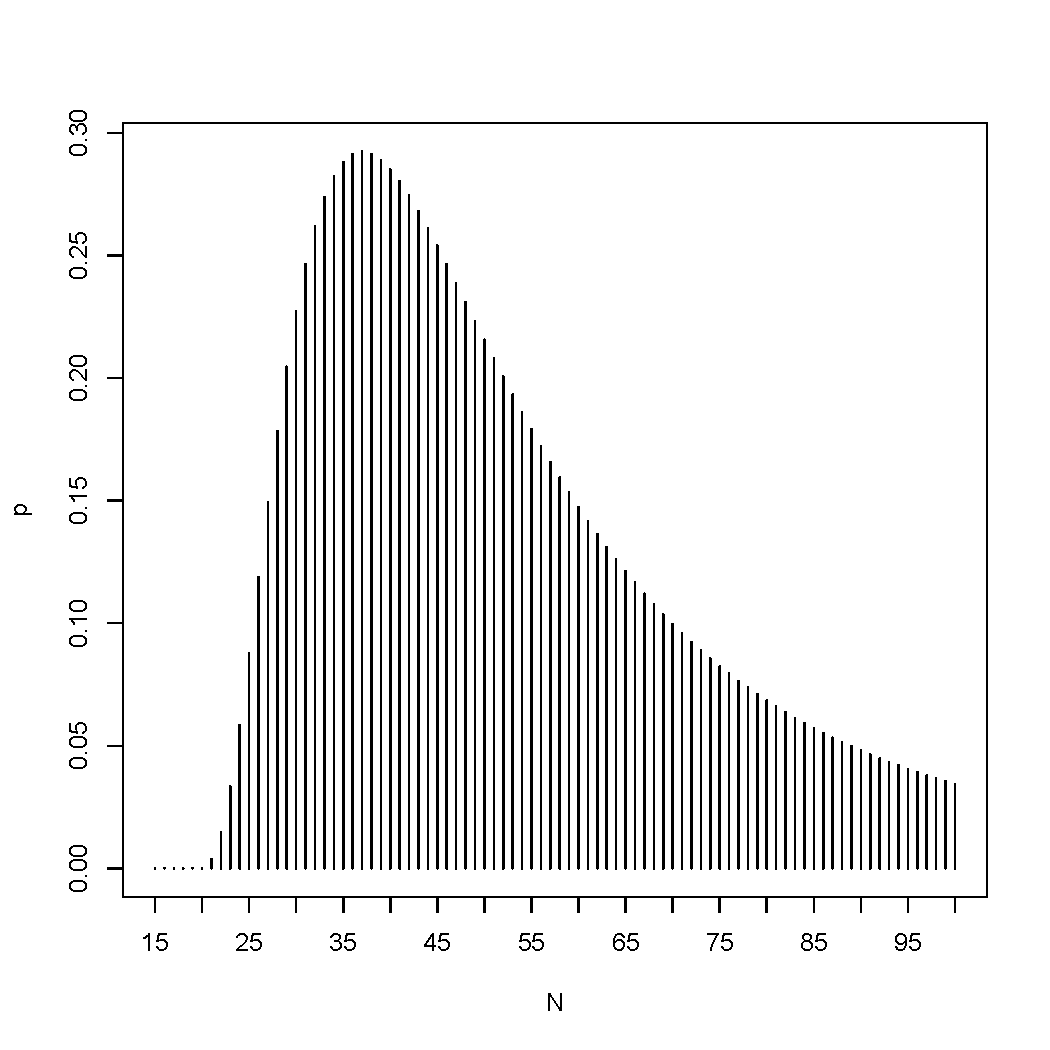
\includegraphics[width=0.65\linewidth]{marca.pdf}
% \end{center}


\end{frame}


\begin{frame}
\frametitle{Ejemplo: Marca-recaptura}

El estimador
$$
\widehat{N}=\frac{n\cdot K}{k}
$$
es sesgado, con sesgo $\tendeix 0$
\bigskip

El \emph{estimador de Chapman}
$$
\widehat{N}=\frac{(n+1)\cdot (K+1)}{k+1}-1
$$
es menos segado para  muestras pequeñas, y no sesgado si $K+n\geq N$ (pero no máximo verosímil)
\end{frame}


\end{document}



